\section{Frequenzgang des invertierenden Verstärkers}
In diesem Versuch wird ein invertierender Operationsverstärker  für unterschiedliche Sollverstärkungen untersucht. Der schematische Aufbau findet sich in der Abbildung\ref{fig:aufbau1}.
\begin{figure}[h]
    \centering
    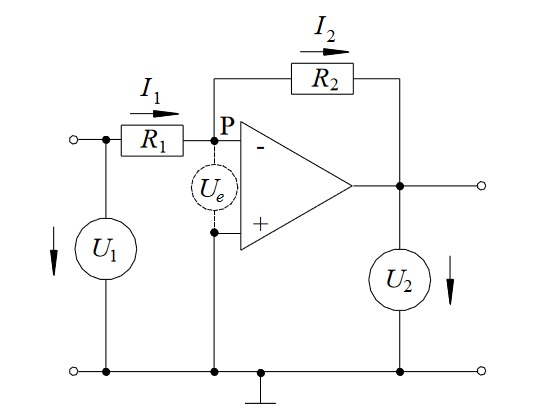
\includegraphics[width=0.5\textwidth]{versuch1/aufbauv1.png}
    \caption{Schematischer Aufbau des Versuches, entnommen aus \cite{script}}
    \label{fig:aufbau1}
\end{figure}
Der Operationsverstärker wird hierbei mit einer Plus-Minus-Spannung von 12 V betrieben. Der Eingangswiderstand $R_1=1$ $k\Omega$ bleibt während des gesamten Versuches konstant, während der Rückkopplungswiderstand $R_2$ variiert wird. Es wird mit einem Funktionsgenerator ein Sweep durchgeführt, welcher an der Klemmspannung $U_1$ angelegt ist und eine Amplitude von 100 mV, einen DC-Offset von 0 V und eine Sweepzeit von $\Delta t$=2,5 s besitzt. Der Sweep läuft von einer Frequenz f von 1 kHz bis 400 kHz, wobei bei jedem $R_2$ ein anderer Bereich betrachtet wird, nämlich von 1 kHz bis zu:
\begin{itemize}[noitemsep,nosep]
	\item 400 kHz bei 5 $k\Omega$
	\item 200 kHz bei 10 $k\Omega$
	\item 150 kHz bei 15 $k\Omega$
	\item 100 kHz bei 20 $k\Omega$
\end{itemize}
Das Ausgangssignal wird mit einer Spitzenwerterfassung gemessen, dann gespeichert und mit einem Matlab-Skript in eine txt-Datei umgewandelt. Die gemessenen t-Werte werden mit der Formel \ref{eqn:formel1} in die benötigten Frequenzwerte f umgerechnet. Dabei ist $f_a$ die Anfangsfrequenz, also 1 kHz und $f_e$ die Endfrequenz des Sweeps, welche geändert wird, je nachdem welches Widerstand verwendet wird.
\begin{equation}\label{eqn:formel1}
    f=f_a+\frac{t}{\Delta t}(f_e-f_a)
\end{equation}
Die gemessenen Spannungswerte müssen noch durch das Eingangssignal, also 100 mV, geteilt werden. Aufgrund der Spitzenwerterfassung gibt es bei den niedrigen Frequenzen einige Messwerte, welche sehr stark von den anderen abweichen. Diese wurden bei den weiteren Berechnungen ignoriert. Die Werte wurden jeweils geplottet und mithilfe einer Funktion aus Gleichung \ref{eqn:formel2} wird jeweils eine Fitfunktion ermittelt.
\begin{equation}\label{eqn:formel2}
    V_r(f)=V_0\frac{1}{\sqrt{1+\biggl(\frac{f}{f_g}\biggr)^2}}
\end{equation}
Dabei sind die Fitparameter $V_0$ die Sollverstärkung und $f_g$ die 3 dB-Grenzfrequenz. Es ergeben sich folgende Fitparameter und Verstärkungs-Bandbreiten Produkte $f_r=V_0f_g$:
\begin{itemize}[noitemsep,nosep]
	\item $V_0=0,0009 \cdot10^4$ und $f_g=5,6135 \cdot10^4$ Hz bei 5 $k\Omega (f_r=5,0522 \cdot 10^3)$
	\item $V_0=0,0009 \cdot10^4$ und $f_g=4,8098 \cdot10^4$ Hz bei 10 $k\Omega (f_r=4,3289 \cdot 10^3)$
	\item $V_0=0,0014 \cdot10^4$ und $f_g=2,4797 \cdot10^4$ Hz bei 15 $k\Omega (f_r=3,4716 \cdot 10^3)$
	\item $V_0=0,0019 \cdot10^4$ und $f_g=1,8665 \cdot10^4$ Hz bei 20 $k\Omega (f_r=3,5464 \cdot 10^3)$
\end{itemize}
Die Messwerte und Fitfunktionen sind in \ref{fig:graphen} dargestellt. Die Verläufe sehen sich recht ähnlich, allerdings unterscheiden sie sich darin, bei welchem Wert sie starten. Der Verlauf in der doppeltlogarithmischen Darstellung sinkt zu Beginn sehr langsam, mit der Zeit wird dieser jedoch immer schneller.
\begin{figure}
    \centering
    \begin{subfigure}[t]{0.45\linewidth}
        \centering
		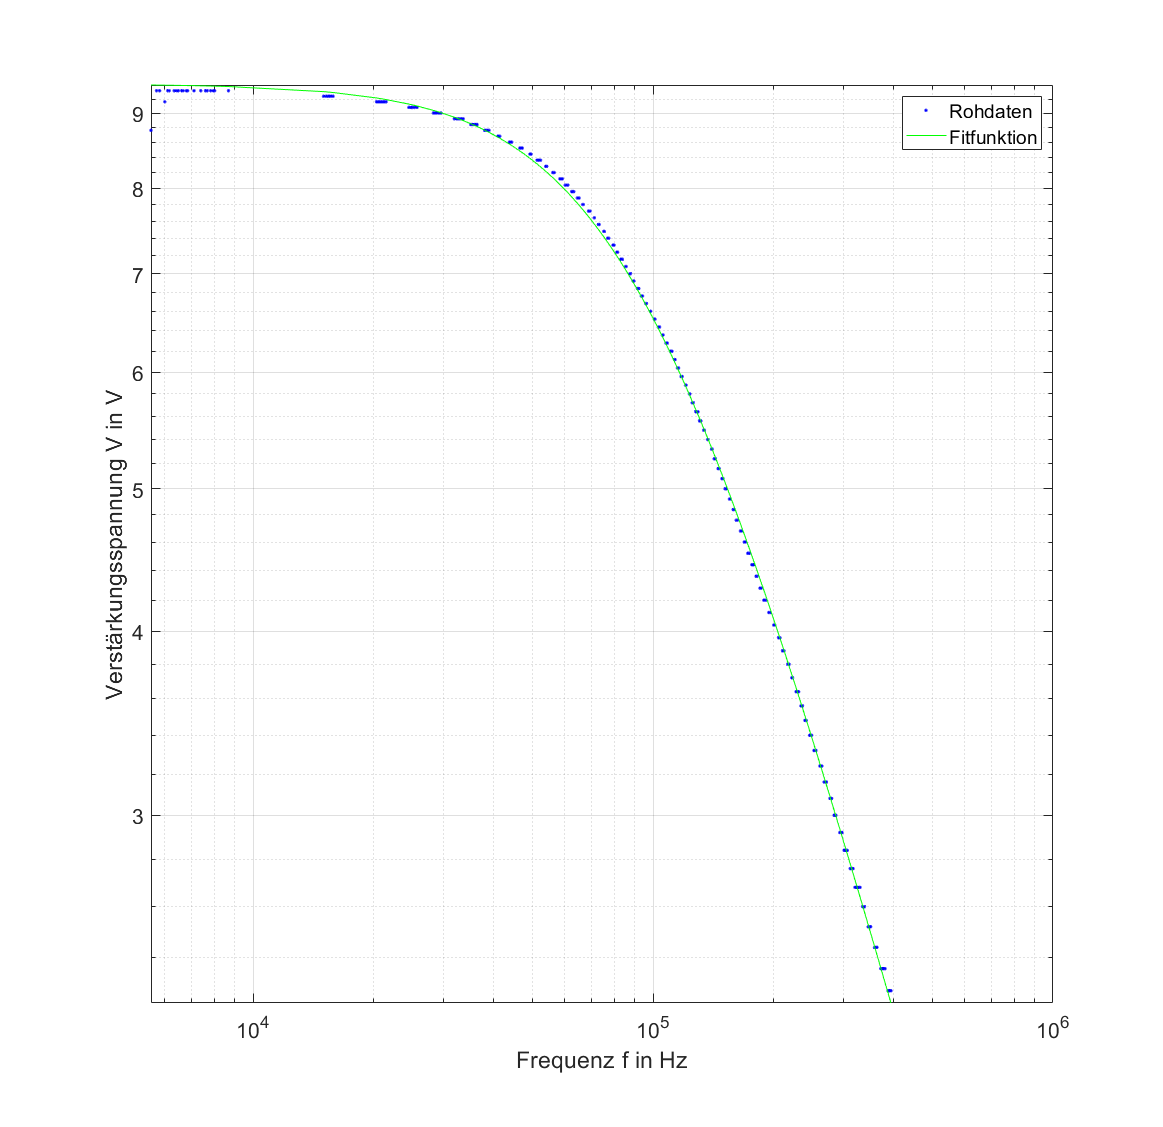
\includegraphics[width=\linewidth]{versuch1/5kOhm.png}
		\caption{$R_2=5$ $k \Omega$}
    \end{subfigure}
\hfill
     \begin{subfigure}[t]{0.45\linewidth}
        \centering
		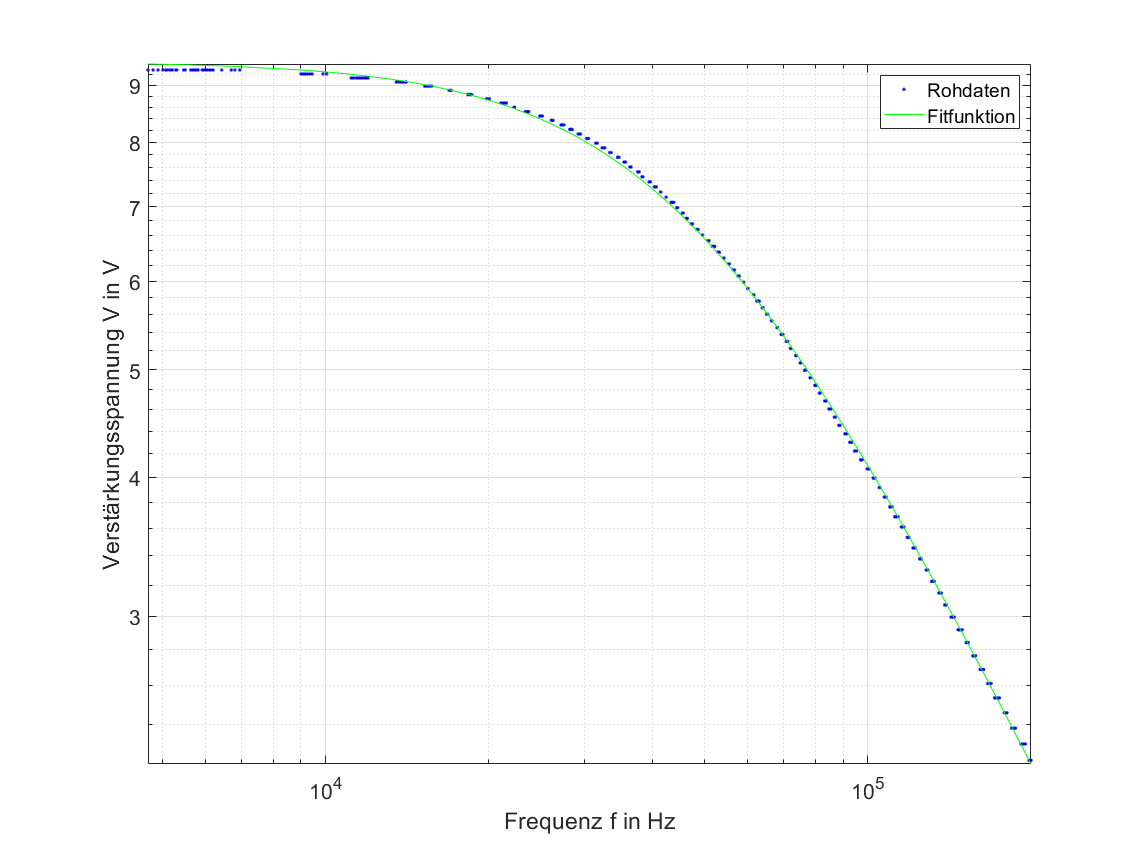
\includegraphics[width=\linewidth]{versuch1/10kOhm.png}
		\caption{$R_2=10$ $k \Omega$}
    \end{subfigure}

     \begin{subfigure}[t]{0.45\linewidth}
        \centering
		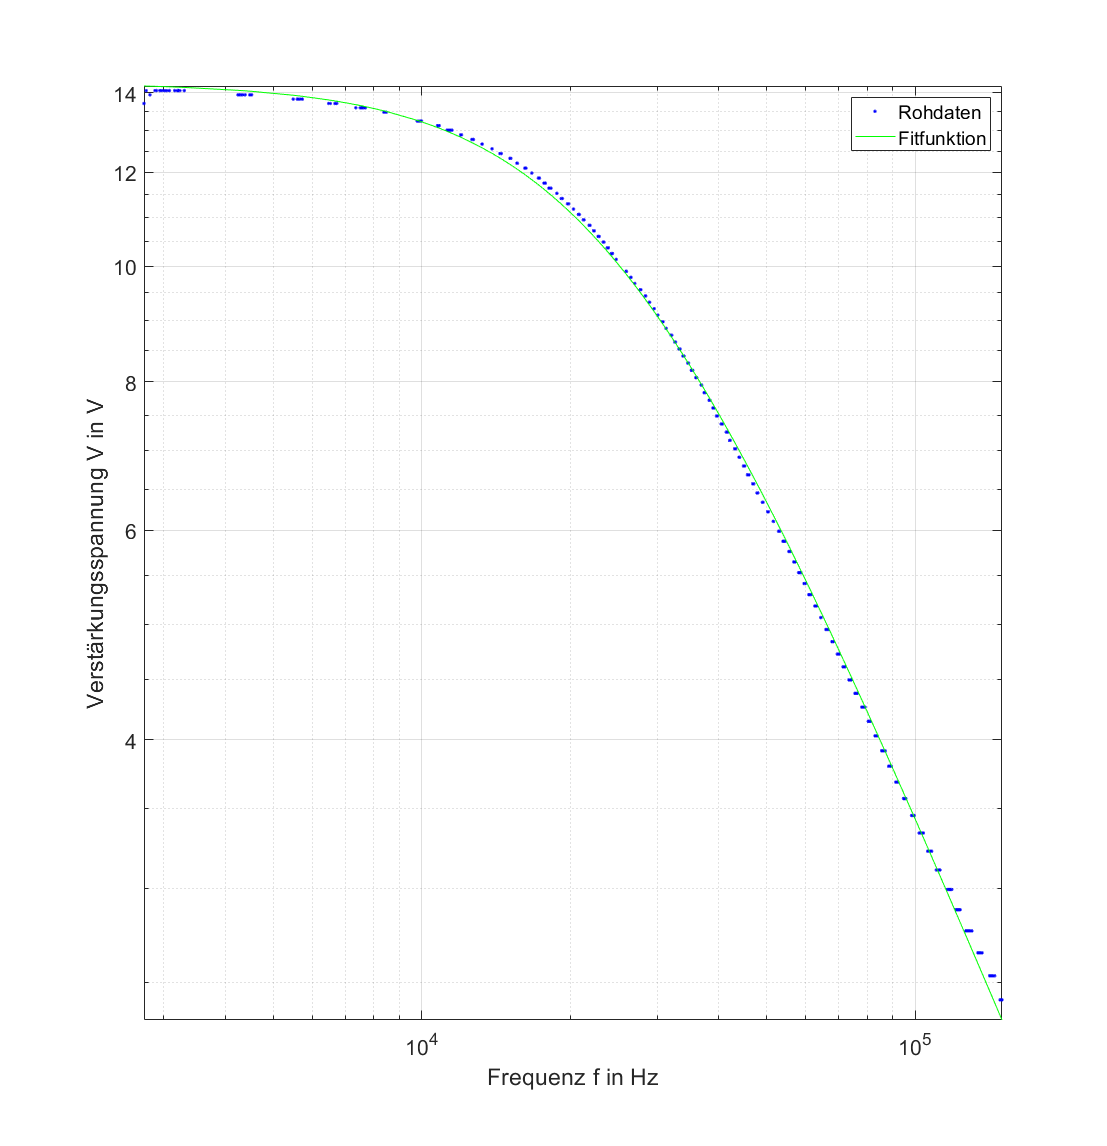
\includegraphics[width=\linewidth]{versuch1/15kOhm.png}
		\caption{$R_2=15$ $k \Omega$}
    \end{subfigure}
\hfill
     \begin{subfigure}[t]{0.45\linewidth}
        \centering
		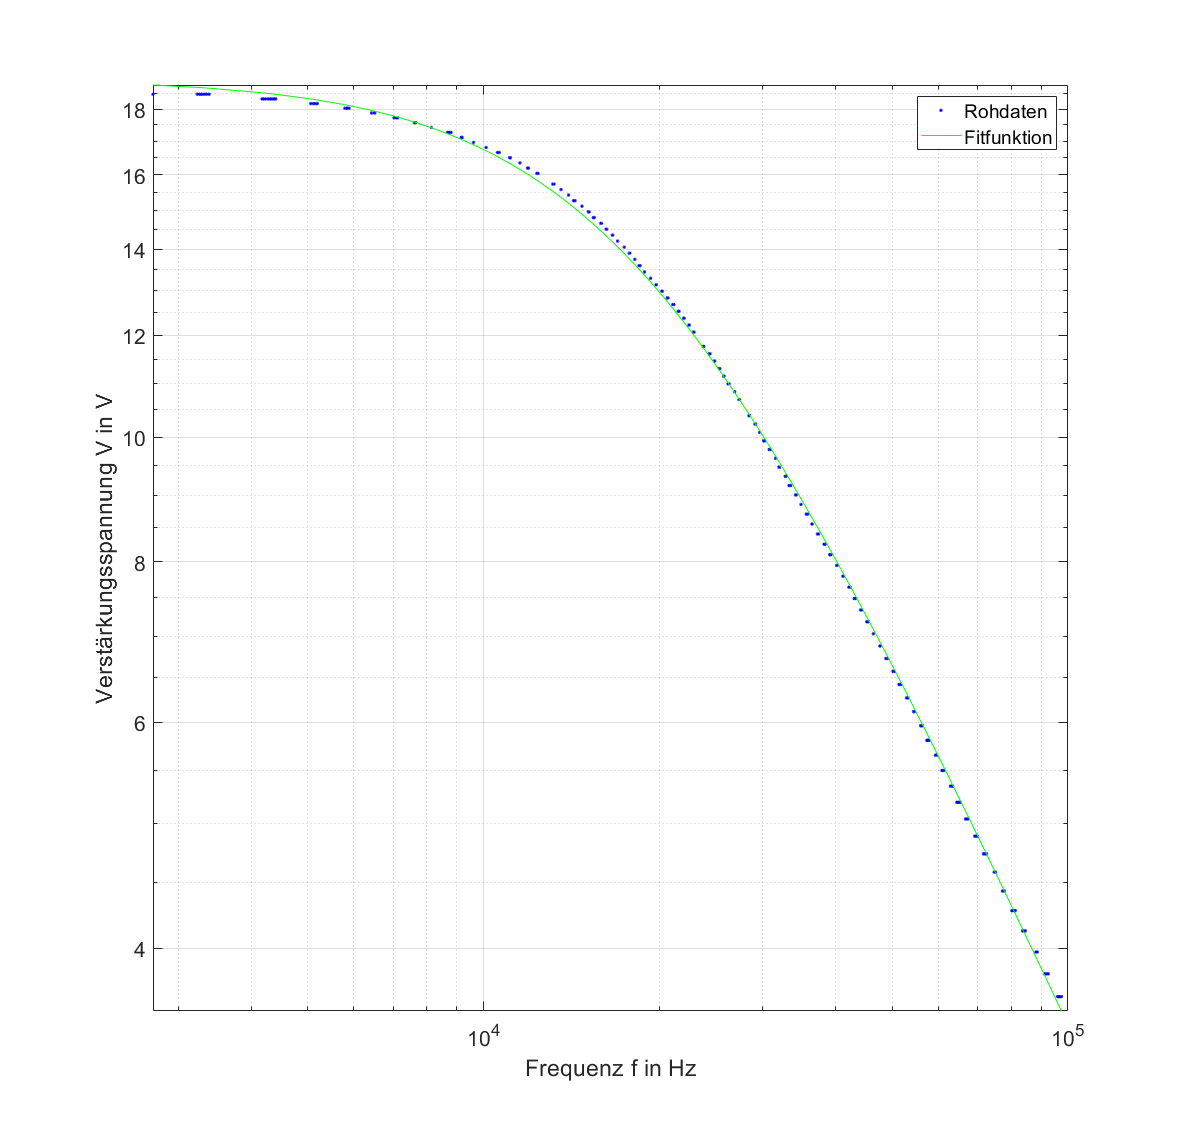
\includegraphics[width=\linewidth]{versuch1/20kOhm.png}
		\caption{$R_2=20$ $k \Omega$}
    \end{subfigure}
    \caption{Darstellung der Messwerte und Fitfunktionen für alle $R_2$}
    \label{fig:graphen}
\end{figure}